\section{Results}

\\
\subsection{Speed-Up}

\subsection{Data Transfer Overhead}
This subsection presents and descibes the results obtained by running matrix multiplication on a NVDIA GeForce GT435M GPU using the OpenCL interface. The run times measured in this subsection exclude the overhead time (the time taken to write data from the CPU and the time taken to read data from the GPU once calculations have been completed). 
\\
The table below summaries the full subset of results and shows the run time 
\begin{center}
	\begin{tabular}{||c c c||} 
		\hline
		Square Matrix Size, N &  Run Time/ms & Speed Up Factor \\ [0.1ex] 
		\hline\hline
		2 &	0.0023241 & 0,002\\
		\hline
		22 & 0,029837 & 0,201\\
		\hline
		42 & 0,039847 & 1,170\\
		\hline
		62 & 0,047434 & 3,542\\
		\hline
		82 & 0,04578 & 7,033\\
		\hline
		102	& 0,083729 & 9,26\\
		\hline
	    122	& 0,100274 & 16,40\\
		\hline
		142	& 0,144703 & 21,75\\
		\hline
		162	& 0,182872 & 26,32\\
		\hline
		182	& 0,261559 & 28,41\\
		\hline
		
	\end{tabular}
\end{center}

The relationship between run time and the square matrix size ,N is shown in the graph below.
\\
\vspace{2mm}
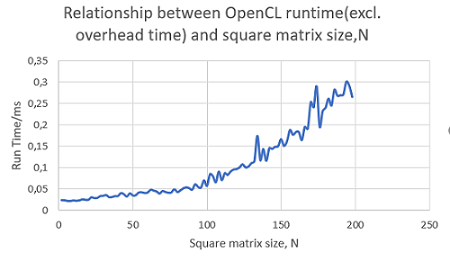
\includegraphics{Figures/part2.PNG}

\subsection{Processing Delay}
When the experiment in part 1 was run without including the OpenClWrteData and OpenCLReadData functions, a much smaller run time was obtained. This runtime was subtracted from the run time time obtained in part 1 to calculate the processing delay. 

\vspace{2mm}
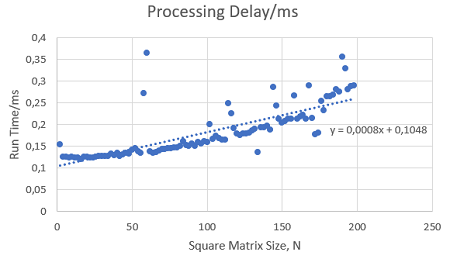
\includegraphics{Figures/processing_delay.PNG}

From the figure above, it can be seen that the processing delay is directly proportional to the Matric size, N.
\\
\vspace{2mm}
